% F02 (CVPR-Figure draft). Conceptual; row (b) image is an observed merged-cluster frame.
\begin{figure}[t]
\centering
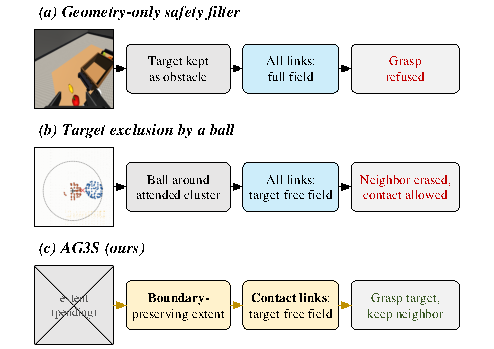
\includegraphics[width=\linewidth]{figures/fig02_overview/cvprfig/out/fig02_overview.pdf}
\caption{\textbf{Finding the target is not enough; its boundary decides contact.}
(a) Treating the target as an obstacle blocks the grasp. (b) Removing a ball around the attended
cluster also erases a touching neighbor, so contact with it is allowed. (c) AG3S keeps the
target's observed boundary and applies the exemption only to the contact links.}
\label{fig:overview}
\end{figure}
